%% LyX 2.2.2 created this file.  For more info, see http://www.lyx.org/.
%% Do not edit unless you really know what you are doing.
\documentclass[brazil]{beamer}
\usepackage{mathptmx}
\usepackage[T1]{fontenc}
\usepackage[latin9]{inputenc}
\synctex=-1
\usepackage{babel}
\usepackage{array}
\usepackage{longtable}
\usepackage{booktabs}
\usepackage{multirow}
\usepackage{amsmath}
\usepackage{amssymb}
\usepackage{graphicx}
\usepackage{setspace}
\ifx\hypersetup\undefined
  \AtBeginDocument{%
    \hypersetup{unicode=true}
  }
\else
  \hypersetup{unicode=true}
\fi

\makeatletter

%%%%%%%%%%%%%%%%%%%%%%%%%%%%%% LyX specific LaTeX commands.
%% Because html converters don't know tabularnewline
\providecommand{\tabularnewline}{\\}

%%%%%%%%%%%%%%%%%%%%%%%%%%%%%% Textclass specific LaTeX commands.
 % this default might be overridden by plain title style
 \newcommand\makebeamertitle{\frame{\maketitle}}%
 % (ERT) argument for the TOC
 \AtBeginDocument{%
   \let\origtableofcontents=\tableofcontents
   \def\tableofcontents{\@ifnextchar[{\origtableofcontents}{\gobbletableofcontents}}
   \def\gobbletableofcontents#1{\origtableofcontents}
 }

%%%%%%%%%%%%%%%%%%%%%%%%%%%%%% User specified LaTeX commands.
\usetheme{Warsaw}
% or ...

\setbeamercovered{transparent}
% or whatever (possibly just delete it)

\makeatother

\begin{document}


\title[Theoretical based RER misalignment estimates.]{Addressing econometric issues on how to construct theoretical based
exchange rate misalignment estimates: searching for a comprehensive
approach.}

\author[Mar�al et. alii. - Sao Paulo School of Economics ]{Emerson Fernandes Mar�al\\
Diogo de Prince\\
Giovanni Merlin\\
Beatrice Zimmermann\\
}

\institute[emerson.marcal@fgv.br]{Sao Paulo School of Economics, FGV \\
WTO Chair Programme\\
}

\makebeamertitle
%\pgfdeclareimage[height=0.5cm]{institution-logo}{cemap_logo}


%\logo{\pgfuseimage{institution-logo}}

\pgfdeclareimage[height=1.5cm]{institution-logo}{logo-conjunto.png}


%\pgfdeclareimage[height=1.5cm]{institution-logo}{C:\Users\emerson.marcal\Dropbox\FGV\CEMAP\pesquisas\observatorio\TB-NFA-approach\apresentacao\FGV-seminario-2017-08-24\logo-conjunto.png}



\logo{\pgfuseimage{institution-logo}}

\AtBeginSubsection[]{

  \frame<beamer>{ 

   \frametitle{Talking Points}   

  \tableofcontents[currentsection,currentsubsection] 

}

}

\beamerdefaultoverlayspecification{<+->}
\begin{frame}{Talking points}

\tableofcontents{}

\end{frame}

\section{CEMAP: }
\begin{frame}{Center for Applied Macroeconomic Research}
\begin{itemize}
\item Center for Applied Macroeconomic Research is part of Sao Paulo School
of Economics;
\item The main goal of the Center is to boost Applied Macroeconomic Research
at the School;
\item Our web-page is \href{http://www.cemap.fgv.br/}{www.cemap.fgv.br/};
\end{itemize}
\end{frame}

\begin{frame}{Our projects}

\begin{itemize}
\item Observatory on Exchange Rate;
\item Forecast Lab;
\item Spatial Econometrics;
\item Reconstructing time series;
\end{itemize}
\end{frame}


\section{Motivation and Goals}

\subsection{Exchange rate misalignment: what and why it is important.}
\begin{frame}{Exchange Rate Misalignment definition and relevance:}

\begin{itemize}
\item<1-> Effective exchange rate misalignment:

\begin{itemize}
\item<1-> Deviations from a long run macroeconomic equilibrium
\item<1-> Economic discussion to define this equilibrium;
\item<1-> Empirical questions about how to estimate this equilibrium;
\end{itemize}
\item<2-> Exchange rate misalignment can:

\begin{itemize}
\item<2-> be related to financial crisis;
\item<2-> permanently influence trade flows;
\item<2-> a sign of serious macroeconomic imbalances;
\end{itemize}
\end{itemize}
\end{frame}

\begin{frame}{Exchange Rate Misalignment: Usual approaches}

\begin{itemize}
\item {\tiny{}Current Account Norm}

\begin{itemize}
\item {\tiny{}Current account Targets: Level of real exchange rate that
guarantees some target level of current account results is obtained;}{\tiny \par}
\item {\tiny{}NFA stabilization Norm: Current account Level that stabilizes
NFA;}{\tiny \par}
\item {\tiny{}Need to estimate elasticity of trade (exports and imports)
to real exchange rate;}{\tiny \par}
\item {\tiny{}Address aggregate consistence;}{\tiny \par}
\end{itemize}
\item {\tiny{}Stability of NFA}

\begin{itemize}
\item {\tiny{}Stability of NFA: Real exchange rate necessary to reach some
NFA level;}{\tiny \par}
\item {\tiny{}Real exchange rate necessary to reach some NFA level;}{\tiny \par}
\item {\tiny{}It can be seen as a minimum prudential level to avoid current
account imbalances;}{\tiny \par}
\item {\tiny{}Simplicity and transparency;}{\tiny \par}
\end{itemize}
\end{itemize}
\end{frame}


\subsection{Traditional Behavioral Exchange Rate Approach}
\begin{frame}{Basic Equilibrium Equation for RER.}

\begin{itemize}
\item {\footnotesize{}From many intertemporal macroeconomic models it's
possible to obtain the following steady state equations}{\footnotesize \par}
\end{itemize}
{\footnotesize{}
\begin{eqnarray}
\overline{RER} & = & -\phi\overline{tb}+\lambda\overline{X}\label{eq:TB-1}
\end{eqnarray}
}{\footnotesize \par}
\begin{itemize}
\item {\footnotesize{}equation \eqref{eq:TB-1} shows that if a country
can run a trade deficit in equilibrium the RER has to appreciate ;}{\footnotesize \par}
\item {\footnotesize{}The term X accounts for any other factor affecting
equilibrium Real Effective Exchange Rate (RER) such as Balassa-Samuelson
effect, terms of trade, government consumption, trade and financial
openness among others;}{\footnotesize \par}
\end{itemize}

\pause{}

{\footnotesize{}
\begin{eqnarray}
\overline{tb} & = & -r*\overline{NFA}\label{eq:TB}
\end{eqnarray}
}{\footnotesize \par}
\begin{itemize}
\item {\footnotesize{}equation \eqref{eq:TB} shows that a country can run
a trade deficits if revenues from NFA are large enough;}{\footnotesize \par}
\end{itemize}
\end{frame}

\begin{frame}{A brief description of traditional BEER approach}

\begin{itemize}
\item {\footnotesize{}Fundamental Real exchange rate is calculated using
an econometric model (based on \eqref{eq:TB}):}

{\footnotesize{}Applications: Faruquee \cite{faruqee1994long}, Clark
\cite{clark1999exchange}, Ubide \cite{ubide1999global} and Kubota
\cite{kubota2009real}}{\footnotesize \par}
\item<1-> {\footnotesize{}Cointegration techniques based on selected series
associated with fundamentals ;}{\footnotesize \par}
\item<2-> {\footnotesize{}Econometric Questions: }{\footnotesize \par}
\item<2-> {\footnotesize{}Detect long run relationship - cointegration analysis;}

\begin{itemize}
\item<2-> {\footnotesize{}Different set of fundamentals can be tested;}{\footnotesize \par}
\end{itemize}
\item<3-> {\footnotesize{}Perform permanent and transitory decomposition to
better understand the adjustment towards equilibrium;}

\begin{itemize}
\item<4-> {\footnotesize{}Gonzalo and Granger decomposition \cite{gonzalo1995estimation}
is the most common choice;}{\footnotesize \par}
\end{itemize}
\end{itemize}
\end{frame}

\begin{frame}{Motivation and goals}

\begin{itemize}
\item<1-> {\small{}Highlight the importance of jointly modeling RER, trade
balances and net foreign asset and not only RER;}

\begin{itemize}
\item<2-> {\small{}Test long run over-identifying restrictions;}{\small \par}
\item<3-> {\small{}Decompose exchange rate misalignment into economically meaningful
parts;}{\small \par}
\item<4-> {\small{}Check if RER has a drift or not;}{\small \par}
\item<5-> {\small{}Discuss when the trade balance information is not useful
for addressing misalignment}{\small \par}
\item<6-> {\small{}Extend Blinder-Oaxaca Decomposition \cite{blinder1973wage}
to our problem;}{\small \par}
\end{itemize}
\end{itemize}
\end{frame}


\section{Addressing Important Econometric Issues}

\subsection{Our approach: Joint Modeling (JMA)}
\begin{frame}{Our starting point}

\begin{itemize}
\item<1-> {\small{}We assume for simplicity but test that DGP for the variables
trade balance, real effective exchange rate and net foreign asset
position and fundamentals is given by the following vector autoregressive
model:
\begin{equation}
\Delta Y_{t}=\Gamma_{1}\Delta Y_{t-1}+...+\Gamma_{k-1}\Delta Y_{t-k+1}+\alpha\beta'Y{}_{t-1}+\mu+\varepsilon_{t}\label{eq:vecm}
\end{equation}
}{\small \par}
\item<2-> {\small{}Instead of arbitrarily ignoring trade balance information
and estimate \eqref{eq:TB}, we jointly estimate \eqref{eq:TB} and
\eqref{eq:TB-1}.}{\small \par}
\item<3-> {\small{}We use long run restrictions suggested by the theory to
validate the exchange rate misalignment estimate;}{\small \par}
\end{itemize}
\end{frame}

\begin{frame}{Transitory and Permanent components}

\begin{itemize}
\item {\scriptsize{}Using the parameters from \eqref{eq:vecm}, it is possible
to calculate the transitory ($T_{it}$) and permanent ($P_{it}$)
components from the following equations:
\begin{eqnarray}
P_{t} & = & \beta_{\perp}(\alpha_{\perp}'\beta_{\perp})^{-1}\alpha_{\perp}'Y_{t}\label{eq:pt}
\end{eqnarray}
\begin{align}
T_{t} & =\alpha(\beta'\alpha)^{-1}\beta'Y_{t}\label{eq:tt}
\end{align}
}{\scriptsize \par}
\end{itemize}

\pause{}
\begin{itemize}
\item {\scriptsize{}Assuming that the real exchange rate is in the first
position of the vector, and using the value of the error correction
mechanism centered on their own means, we can calculate the misalignment
using the following equation, then}\textrm{\scriptsize{}:}{\scriptsize{}
\begin{align}
mis_{t} & \equiv F{}_{1}(\beta_{1}'Y_{t}-E([\beta_{1}'Y_{t}])+F{}_{2}(\beta_{2}'Y{}_{t}-E([\beta_{2}'Y_{t}])\label{eq:GG-domestico-1-1}
\end{align}
}{\scriptsize \par}
\end{itemize}
\textrm{\scriptsize{}where $[\begin{array}{cc}
V_{1} & V_{2}\end{array}]=(\beta'\alpha)^{-1}$ and $V_{i}$ has dimension 2x1}{\scriptsize \par}

\textrm{\scriptsize{}$F\equiv[F_{1}F_{2}]=[\begin{array}{cc}
[\begin{array}{cccc}
1 & 0 & ... & 0\end{array}][\begin{array}{cc}
\alpha_{1} & \alpha_{2}\end{array}]V_{1} & [\begin{array}{cccc}
1 & 0 & ... & 0\end{array}][\begin{array}{cc}
\alpha_{1} & \alpha_{2}\end{array}]V_{2}\end{array}]$}\textrm{.}

\end{frame}


\subsection{Long run identifying restrictions and exchange rate misalignment
decomposition}
\begin{frame}{Are theoretical based restrictions valid? Test}

\begin{itemize}
\item \textbf{How to check identification restrictions of the theoretical model?}

\begin{itemize}
\item \textrm{\footnotesize{}Assume that the following sets of variable
are modeled:
\[
Y_{t}=\begin{bmatrix}rer & tb & nfa & Fund1 & Fund2\end{bmatrix}^{'}
\]
}{\footnotesize{}where $Fund1$ and $Fund2$ are any variables related
to fundamentals.}{\footnotesize \par}
\item \textrm{\footnotesize{}If over-identifying restrictions hold, then
the cointegrated vectors satisfy \eqref{eq:beta1-1}: 
\begin{eqnarray}
\beta_{r'} & = & \begin{bmatrix}1 & 0 & b_{31} & b_{41} & b_{51}\\
0 & 1 & b_{32} & 0 & 0
\end{bmatrix}^{'}\label{eq:beta1-1}
\end{eqnarray}
}{\footnotesize{}where }\textrm{\footnotesize{}$\gamma=\{b_{31},b_{32},b_{41},b_{51}\}$
are the coefficients of the long run relationship to be estimated}{\footnotesize{}.}{\footnotesize \par}
\end{itemize}
\end{itemize}
\end{frame}

\begin{frame}{Does RER have a drift?}

\begin{itemize}
\item \textbf{How to test that RER is not drifting?}

\begin{itemize}
\item {\footnotesize{}\eqref{eq:vecm} should satisfy:}\textrm{\footnotesize{}
\begin{eqnarray}
\mu & = & \alpha\varphi\label{eq:mu=00003Dalpha}
\end{eqnarray}
}{\footnotesize{}where }\textrm{\footnotesize{}$\varphi$ is a matrix
of order r x 1 and r is the number of cointegrated relationship in
the system.}{\footnotesize \par}
\end{itemize}
\end{itemize}
\end{frame}


\subsection{Why exchange misalignment can differ.}
\begin{frame}{Adapting Blinder-Oaxaca decomposition:}

\begin{itemize}
\item \textbf{Blinder-Oaxaca decomposition (\cite{blinder1973wage,oaxaca1973male}).}
\end{itemize}
\textrm{
\begin{equation}
\begin{array}{ccc}
mis_{i,t}^{JMA}-mis_{i,t}^{BEER}= & \underset{Less\:weight\:on\:what\:we\:knew}{\underbrace{(\frac{h_{1}^{JMA}}{h_{1}^{BEER}}-1)(h_{1}^{BEER}f_{1,t}^{BEER})}}+\\
 & +\underset{What\:we\:learn\:from\:new\:model}{\underbrace{h_{1}^{JMA}(f_{1,t}^{JMA}-f_{1,t}^{BEER})+h_{2}^{JMA}f_{2,t}^{JMA}}}
\end{array}
\end{equation}
}
\end{frame}

\begin{frame}{Adapting Blinder-Oaxaca decomposition:}

\begin{itemize}
\item If cointegrated relationships are properly identified:
\end{itemize}
\textrm{
\begin{equation}
f_{1,t}^{JMA}-f_{1,t}^{BEER}\overset{p}{\rightarrow}0
\end{equation}
}
\begin{itemize}
\item \textrm{Both models are nested and it is interesting to investigate
whether}
\begin{itemize}
\item \textrm{$\frac{h_{1}^{JMA}}{h_{1}^{BEER}}=1$}
\item \textrm{$h_{2}^{JMA}=0$.}
\end{itemize}
\end{itemize}
\textrm{.}
\end{frame}

\begin{frame}{Conditions to guarantee \textrm{$h_{2}^{JMA}=0$}}

\begin{itemize}
\item Weight of GG decomposition are given by:

\end{itemize}
\textrm{
\begin{equation}
\begin{bmatrix}h_{1}^{JMA} & h_{2}^{JMA}\end{bmatrix}=\alpha(\beta'\alpha)^{-1}=\begin{bmatrix}\alpha_{11} & \alpha_{21}\\
\alpha_{12} & \alpha_{22}
\end{bmatrix}\begin{pmatrix}\beta'_{1}\alpha_{1} & \beta'_{1}\alpha_{2}\\
\beta'_{2}\alpha_{1} & \beta'_{2}\alpha_{2}
\end{pmatrix}^{-1}
\end{equation}
}
\begin{itemize}
\item If \textrm{$\beta'_{1}\alpha_{2}=0$ and $\alpha_{21}=0$ then $h_{2}^{JMA}=0$. }
\item \textrm{Note that $\alpha_{21}=0$ is not sufficient to guarantee
$h_{2}^{JMA}=0$. }
\end{itemize}
\end{frame}

\begin{frame}{Example when \textrm{$h_{2}^{JMA}=0$}}

\begin{itemize}
\item Assume that:

\end{itemize}
\textrm{
\begin{equation}
\alpha^{'}=\begin{bmatrix}\alpha_{11} & ab_{32} & -a & \alpha_{41} & \alpha_{51}\\
0 & \alpha_{21} & \alpha_{31} & \alpha_{41} & \alpha_{51}
\end{bmatrix}
\end{equation}
}

\textrm{.
\begin{eqnarray}
\beta' & = & \begin{bmatrix}1 & 0 & b_{31} & b_{41} & b_{51}\\
0 & 1 & b_{32} & 0 & 0
\end{bmatrix}
\end{eqnarray}
}
\begin{itemize}
\item Then \textrm{$\beta'_{1}\alpha_{2}=0$ and $\alpha_{21}=0$ and so
$h_{2}^{JMA}=0$. }
\end{itemize}
\end{frame}

\begin{frame}{Example when \textrm{$(\frac{h_{1}^{JMA}}{h_{1}^{BEER}}-1)=0$ and
$h_{2}^{JMA}=0$}}

\begin{itemize}
\item Assume that:

\end{itemize}
\textrm{
\begin{equation}
\alpha^{'}=\begin{bmatrix}\alpha_{11} & 0 & 0 & 0 & 0\\
0 & 0 & \alpha_{31} & \alpha_{41} & \alpha_{51}
\end{bmatrix}
\end{equation}
}

\textrm{.
\begin{eqnarray}
\beta' & = & \begin{bmatrix}1 & 0 & b_{31} & b_{41} & b_{51}\\
0 & 1 & b_{32} & 0 & 0
\end{bmatrix}
\end{eqnarray}
}
\begin{itemize}
\item Then \textrm{$(\frac{h_{1}^{JMA}}{h_{1}^{BEER}}-1)=0$ and $h_{2}^{JMA}=0$}.
Note also that\textrm{ $h_{1}^{JMA}=h_{1}^{BEER}=1$}
\end{itemize}
\end{frame}


\section{Empirical Illustrations}

\subsection{Database Description}
\begin{frame}{Database description}
\begin{overprint}
\onslide<1> 

{\scriptsize{}}%
\begin{tabular}{|>{\raggedright}p{2.5cm}||>{\raggedright}p{1.5cm}||>{\raggedright}p{5.5cm}|}
\hline 
{\scriptsize{}Variable} & {\scriptsize{}Source} & {\scriptsize{}Definition}\tabularnewline
\hline 
\textcolor{blue}{\scriptsize{}Real Effective Exchange Rate} & \textcolor{blue}{\scriptsize{}IMF and BIS} & \textcolor{blue}{\scriptsize{}Weighted Average of Real exchange rate
based on Consumer price index ($RER_{i,t}$).}\tabularnewline
\hline 
\end{tabular}{\scriptsize \par}
\onslide<2> 

{\scriptsize{}}%
\begin{tabular}{|>{\raggedright}p{2.5cm}||>{\raggedright}p{1.5cm}||>{\raggedright}p{5.5cm}|}
\hline 
{\scriptsize{}Variable} & {\scriptsize{}Source} & {\scriptsize{}Definition}\tabularnewline
\hline 
{\scriptsize{}Real Effective Exchange Rate} & {\scriptsize{}IMF and BIS} & {\scriptsize{}Weighted Average of Real exchange rate based on Consumer
price index ($RER_{i,t}$).}\tabularnewline
\hline 
\textcolor{blue}{\scriptsize{}Trade balance as Share of GDP } & \textcolor{blue}{\scriptsize{}IMF and WB} & \textcolor{blue}{\scriptsize{}Ratio of trade balance and GDP ($TB_{i,t}$)}\tabularnewline
\hline 
\end{tabular}{\scriptsize \par}
\onslide<3> 

{\scriptsize{}}%
\begin{tabular}{|>{\raggedright}p{2.5cm}||>{\raggedright}p{1.5cm}||>{\raggedright}p{5.5cm}|}
\hline 
{\scriptsize{}Variable} & {\scriptsize{}Source} & {\scriptsize{}Definition}\tabularnewline
\hline 
{\scriptsize{}Real Effective Exchange Rate} & {\scriptsize{}IMF and BIS} & {\scriptsize{}Weighted Average of Real exchange rate based on Consumer
price index ($RER_{i,t}$).}\tabularnewline
\hline 
{\scriptsize{}Trade balance as Share of GDP } & {\scriptsize{}IMF and WB} & {\scriptsize{}Ratio of trade balance and GDP ($TB_{i,t}$)}\tabularnewline
\hline 
\textcolor{blue}{\scriptsize{}Relative per capita income} & \textcolor{blue}{\scriptsize{}WB} & \textcolor{blue}{\scriptsize{}$BSPIB_{i,t}=\frac{Percapita\:Indexi_{i,t}}{\sum_{i=1}^{N}w_{i}Percapita\:Index_{j,t}}$}\tabularnewline
\hline 
\end{tabular}{\scriptsize \par}
\onslide<4> 

{\scriptsize{}}%
\begin{tabular}{|>{\raggedright}p{2.5cm}||>{\raggedright}p{1.5cm}||>{\raggedright}p{5.5cm}|}
\hline 
{\scriptsize{}Variable} & {\scriptsize{}Source} & {\scriptsize{}Definition}\tabularnewline
\hline 
{\scriptsize{}Real Effective Exchange Rate} & {\scriptsize{}IMF and BIS} & {\scriptsize{}Weighted Average of Real exchange rate based on Consumer
price index ($RER_{i,t}$).}\tabularnewline
\hline 
{\scriptsize{}Trade balance as Share of GDP } & {\scriptsize{}IMF and WB} & {\scriptsize{}Ratio of trade balance and GDP ($TB_{i,t}$)}\tabularnewline
\hline 
{\scriptsize{}Relative per capita income} & {\scriptsize{}WB} & {\scriptsize{}$BSPIB_{i,t}=\frac{Percapita\:Indexi_{i,t}}{\sum_{i=1}^{N}w_{i}Percapita\:Index_{j,t}}$}\tabularnewline
\hline 
\textcolor{blue}{\scriptsize{}Relative terms of trade} & \textcolor{blue}{\scriptsize{}IMF} & \textcolor{blue}{\scriptsize{}$Tot_{i,t}=\frac{ToT_{i,t}}{\sum_{i=1}^{N}w_{i}ToT{}_{j,t}}$}\tabularnewline
\hline 
\end{tabular}{\scriptsize \par}
\onslide<5> 

{\scriptsize{}}%
\begin{tabular}{|>{\raggedright}p{2.5cm}||>{\raggedright}p{1.5cm}||>{\raggedright}p{5.5cm}|}
\hline 
{\scriptsize{}Variable} & {\scriptsize{}Source} & {\scriptsize{}Definition}\tabularnewline
\hline 
{\scriptsize{}Real Effective Exchange Rate} & {\scriptsize{}IMF and BIS} & {\scriptsize{}Weighted Average of Real exchange rate based on Consumer
price index ($RER_{i,t}$).}\tabularnewline
\hline 
{\scriptsize{}Trade balance as Share of GDP } & {\scriptsize{}IMF and WB} & {\scriptsize{}Ratio of trade balance and GDP ($TB_{i,t}$)}\tabularnewline
\hline 
{\scriptsize{}Relative per capita income} & {\scriptsize{}WB} & {\scriptsize{}$BSPIB_{i,t}=\frac{Percapita\:Indexi_{i,t}}{\sum_{i=1}^{N}w_{i}Percapita\:Index_{j,t}}$}\tabularnewline
\hline 
{\scriptsize{}Relative terms of trade} & {\scriptsize{}IMF} & {\scriptsize{}$Tot_{i,t}=\frac{ToT_{i,t}}{\sum_{i=1}^{N}w_{i}ToT{}_{j,t}}$}\tabularnewline
\hline 
\textcolor{blue}{\scriptsize{}Net Foreign Asset Position} & \textcolor{blue}{\scriptsize{}Milesi e Ferreti and IMF} & \textcolor{blue}{\scriptsize{}Ratio of Net Foreign Asset Position
and GDP ($NFA_{i,t}$)}\tabularnewline
\hline 
\end{tabular}{\scriptsize \par}
\onslide<6> 

{\scriptsize{}}%
\begin{tabular}{|>{\raggedright}p{2.5cm}||>{\raggedright}p{1.5cm}||>{\raggedright}p{5.5cm}|}
\hline 
{\scriptsize{}Variable} & {\scriptsize{}Source} & {\scriptsize{}Definition}\tabularnewline
\hline 
{\scriptsize{}Real Effective Exchange Rate} & {\scriptsize{}IMF and BIS} & {\scriptsize{}Weighted Average of Real exchange rate based on Consumer
price index ($RER_{i,t}$).}\tabularnewline
\hline 
{\scriptsize{}Trade balance as Share of GDP } & {\scriptsize{}IMF and WB} & {\scriptsize{}Ratio of trade balance and GDP ($TB_{i,t}$)}\tabularnewline
\hline 
{\scriptsize{}Relative per capita income} & {\scriptsize{}WB} & {\scriptsize{}$BSPIB_{i,t}=\frac{Percapita\:Indexi_{i,t}}{\sum_{i=1}^{N}w_{i}Percapita\:Index_{j,t}}$}\tabularnewline
\hline 
{\scriptsize{}Relative terms of trade} & {\scriptsize{}IMF} & {\scriptsize{}$Tot_{i,t}=\frac{ToT_{i,t}}{\sum_{i=1}^{N}w_{i}ToT{}_{j,t}}$}\tabularnewline
\hline 
\textcolor{black}{\scriptsize{}Net Foreign Asset Position} & \textcolor{black}{\scriptsize{}Milesi e Ferreti and IMF} & \textcolor{black}{\scriptsize{}Ratio of Net Foreign Asset Position
and GDP ($NFA_{i,t}$)}\tabularnewline
\hline 
\textcolor{blue}{\scriptsize{}Relative price ratio} & \textcolor{blue}{\scriptsize{}IMF} & \textcolor{blue}{\scriptsize{}$BS_{i,t}=\frac{\frac{WSP_{i,t}}{IPCi,_{t}}}{\sum_{i=1}^{N}w_{i}\frac{WSP_{i,t}}{CPI_{i,t}}}$}\tabularnewline
\hline 
\end{tabular}{\scriptsize \par}
\end{overprint}
\end{frame}

\begin{frame}{Cointegration Analysis: Trace}

{\tiny{}.}{\tiny \par}

{\tiny{}}%
\begin{tabular}{crrrrrr}
\multirow{1}{*}[0.1cm]{{\tiny{}Countries}} & \multicolumn{1}{c}{{\tiny{}Rank}} & {\tiny{}RER , NFA} & {\tiny{}RER, BSPIB } & {\tiny{}RER, BS } & {\tiny{}RER, TOT } & {\tiny{}RER, TB }\tabularnewline
\midrule
\multirow{1}{*}[0.2cm]{\textcolor{blue}{\tiny{}Australia }} & \textcolor{blue}{\tiny{}r=0 } & \textcolor{blue}{\tiny{}{*}{*}{*} } & \textcolor{blue}{\tiny{}{*}{*} } &  &  & \textcolor{blue}{\tiny{}{*} }\tabularnewline
\midrule
 & \textcolor{blue}{\tiny{}r=1 } &  &  &  &  & \tabularnewline
\midrule
\textcolor{blue}{\tiny{}Austria } & \textcolor{blue}{\tiny{}r=0 } &  & \textcolor{blue}{\tiny{}{*}{*} } & \textcolor{blue}{\tiny{}{*}{*} } & \textcolor{blue}{\tiny{}n.a. } & \tabularnewline
\midrule
 & \textcolor{blue}{\tiny{}r=1 } &  &  &  & \textcolor{blue}{\tiny{}n.a. } & \tabularnewline
\midrule
\textcolor{blue}{\tiny{}Brazil } & \textcolor{blue}{\tiny{}r=0 } & \textcolor{blue}{\tiny{}{*}{*} } &  &  &  & \textcolor{blue}{\tiny{}{*}{*} }\tabularnewline
\midrule
 & \textcolor{blue}{\tiny{}r=1 } &  &  &  &  & \tabularnewline
\midrule
\textcolor{blue}{\tiny{}China } & \textcolor{blue}{\tiny{}r=0 } &  & \textcolor{blue}{\tiny{}{*}{*}{*} } & \textcolor{blue}{\tiny{}{*}{*}{*} } &  & \textcolor{blue}{\tiny{}{*}{*} }\tabularnewline
\midrule
 & \textcolor{blue}{\tiny{}r=1 } &  & \textcolor{blue}{\tiny{}{*}{*} } &  &  & \tabularnewline
\midrule
{\tiny{}Colombia } & {\tiny{}r=0 } &  &  &  &  & \tabularnewline
\midrule
 & {\tiny{}r=1 } &  &  &  &  & \tabularnewline
\bottomrule
\end{tabular}{\tiny \par}
\end{frame}

\begin{frame}{Cointegration Analysis: Trace}

{\tiny{}.}{\tiny \par}

{\tiny{}}%
\begin{tabular}{crrrrrr}
\multirow{1}{*}[0.1cm]{{\tiny{}Countries}} & \multicolumn{1}{c}{{\tiny{}Rank}} & {\tiny{}RER , NFA} & {\tiny{}RER, BSPIB } & {\tiny{}RER, BS } & {\tiny{}RER, TOT } & {\tiny{}RER, TB }\tabularnewline
\midrule
\textcolor{blue}{\tiny{}Denmark } & \textcolor{blue}{\tiny{}r=0 } & \textcolor{blue}{\tiny{}{*} } &  &  &  & \tabularnewline
\midrule
 & \textcolor{blue}{\tiny{}r=1 } &  &  &  &  & \tabularnewline
\midrule
\textcolor{blue}{\tiny{}Finland } & \textcolor{blue}{\tiny{}r=0 } & \textcolor{blue}{\tiny{}{*}{*}{*} } &  & \textcolor{blue}{\tiny{}{*} } &  & \tabularnewline
\midrule
 & \textcolor{blue}{\tiny{}r=1 } &  &  &  &  & \tabularnewline
\midrule
\textcolor{blue}{\tiny{}Germany } & \textcolor{blue}{\tiny{}r=0 } &  &  &  & \textcolor{blue}{\tiny{}{*} } & \textcolor{blue}{\tiny{}{*}{*}{*} }\tabularnewline
\midrule
 & \textcolor{blue}{\tiny{}r=1 } &  &  &  &  & \tabularnewline
\midrule
{\tiny{}Greece } & {\tiny{}r=0 } &  &  &  &  & \tabularnewline
\midrule
 & {\tiny{}r=1 } &  &  &  &  & \tabularnewline
\midrule
{\tiny{}Ireland } & {\tiny{}r=0 } &  &  &  &  & \tabularnewline
\midrule
 & {\tiny{}r=1 } &  &  &  &  & \tabularnewline
\bottomrule
\end{tabular}{\tiny{}.}{\tiny \par}
\end{frame}

\begin{frame}{Cointegration Analysis: Trace}

{\tiny{}.}{\tiny \par}

{\tiny{}}%
\begin{tabular}{crrrrrr}
\multirow{1}{*}[0.1cm]{{\tiny{}Countries}} & \multicolumn{1}{c}{{\tiny{}Rank}} & {\tiny{}RER , NFA} & {\tiny{}RER, BSPIB } & {\tiny{}RER, BS } & {\tiny{}RER, TOT } & {\tiny{}RER, TB }\tabularnewline
\midrule
\textcolor{blue}{\tiny{}Italy } & \textcolor{blue}{\tiny{}r=0 } & \textcolor{blue}{\tiny{}{*} } &  &  &  & \tabularnewline
\midrule
 & \textcolor{blue}{\tiny{}r=1 } &  &  &  &  & \tabularnewline
\midrule
\textcolor{blue}{\tiny{}Japan } & \textcolor{blue}{\tiny{}r=0 } & \textcolor{blue}{\tiny{}{*}{*}{*} } & \textcolor{blue}{\tiny{}{*}{*} } &  & \textcolor{blue}{\tiny{}{*} } & \textcolor{blue}{\tiny{}{*}{*} }\tabularnewline
\midrule
 & \textcolor{blue}{\tiny{}r=1 } & \textcolor{blue}{\tiny{}{*} } &  &  &  & \tabularnewline
\midrule
\textcolor{blue}{\tiny{}Korea } & \textcolor{blue}{\tiny{}r=0 } & \textcolor{blue}{\tiny{}{*}{*}{*} } & \textcolor{blue}{\tiny{}{*}{*}{*} } &  &  & \textcolor{blue}{\tiny{}{*}{*} }\tabularnewline
\midrule
 & \textcolor{blue}{\tiny{}r=1 } &  & \textcolor{blue}{\tiny{}{*}{*}{*} } &  &  & \tabularnewline
\midrule
\textcolor{blue}{\tiny{}Mexico } & \textcolor{blue}{\tiny{}r=0 } &  &  & \textcolor{blue}{\tiny{}{*} } & \textcolor{blue}{\tiny{}{*}{*}{*} } & \textcolor{blue}{\tiny{}{*}{*}{*} }\tabularnewline
\midrule
 & \textcolor{blue}{\tiny{}r=1 } &  &  &  & \textcolor{blue}{\tiny{}{*}{*}{*} } & \textcolor{blue}{\tiny{}{*}{*} }\tabularnewline
\midrule
\textcolor{blue}{\tiny{}Netherlands } & \textcolor{blue}{\tiny{}r=0 } &  & \textcolor{blue}{\tiny{}{*}{*} } & \textcolor{blue}{\tiny{}{*}{*} } &  & \tabularnewline
\midrule
 & \textcolor{blue}{\tiny{}r=1 } &  &  &  &  & \tabularnewline
\bottomrule
\end{tabular}{\tiny \par}
\end{frame}

\begin{frame}{Cointegration Analysis: Trace}

{\tiny{}.}{\tiny \par}

{\tiny{}}%
\begin{tabular}{crrrrrr}
\multirow{1}{*}[0.1cm]{{\tiny{}Countries}} & \multicolumn{1}{c}{{\tiny{}Rank}} & {\tiny{}RER , NFA} & {\tiny{}RER, BSPIB } & {\tiny{}RER, BS } & {\tiny{}RER, TOT } & {\tiny{}RER, TB }\tabularnewline
\midrule
\textcolor{blue}{\tiny{}New Zealand } & \textcolor{blue}{\tiny{}r=0 } & \textcolor{blue}{\tiny{}{*} } &  & \textcolor{blue}{\tiny{}{*} } & \textcolor{blue}{\tiny{}{*}{*} } & \textcolor{blue}{\tiny{}{*} }\tabularnewline
\midrule
 & \textcolor{blue}{\tiny{}r=1 } &  &  &  &  & \tabularnewline
\midrule
\textcolor{blue}{\tiny{}Norway } & \textcolor{blue}{\tiny{}r=0 } & \textcolor{blue}{\tiny{}{*}{*} } &  &  &  & \tabularnewline
\midrule
 & \textcolor{blue}{\tiny{}r=1 } &  &  &  &  & \tabularnewline
\midrule
{\tiny{}Portugal } & {\tiny{}r=0 } &  &  &  & {\tiny{}n.a. } & \tabularnewline
\midrule
 & {\tiny{}r=1 } &  &  &  & {\tiny{}n.a. } & \tabularnewline
\midrule
\textcolor{blue}{\tiny{}Singapore } & \textcolor{blue}{\tiny{}r=0 } & \textcolor{blue}{\tiny{}{*}{*} } & \textcolor{blue}{\tiny{}{*}{*}{*} } &  &  & \textcolor{blue}{\tiny{}{*}{*} }\tabularnewline
\midrule
 & \textcolor{blue}{\tiny{}r=1 } &  & \textcolor{blue}{\tiny{}{*}{*} } &  &  & \textcolor{blue}{\tiny{}{*} }\tabularnewline
\midrule
\textcolor{blue}{\tiny{}Spain } & \textcolor{blue}{\tiny{}r=0 } & \textcolor{blue}{\tiny{}{*}{*}{*} } &  & \textcolor{blue}{\tiny{}{*} } &  & \textcolor{blue}{\tiny{}{*} }\tabularnewline
\midrule
 & \textcolor{blue}{\tiny{}r=1 } &  &  & \textcolor{blue}{\tiny{}{*} } &  & \tabularnewline
\bottomrule
\end{tabular}{\tiny \par}
\end{frame}

\begin{frame}{Cointegration Analysis: Trace}

{\tiny{}.}{\tiny \par}

{\tiny{}}%
\begin{tabular}{crrrrrr}
\multirow{1}{*}[0.1cm]{{\tiny{}Countries}} & \multicolumn{1}{c}{{\tiny{}Rank}} & {\tiny{}RER , NFA} & {\tiny{}RER, BSPIB } & {\tiny{}RER, BS } & {\tiny{}RER, TOT } & {\tiny{}RER, TB }\tabularnewline
\midrule
\textcolor{blue}{\tiny{}Sweden } & \textcolor{blue}{\tiny{}r=0 } & \textcolor{blue}{\tiny{}{*}{*} } &  & \textcolor{blue}{\tiny{}{*}{*} } &  & \tabularnewline
\midrule
 & \textcolor{blue}{\tiny{}r=1 } &  &  &  &  & \tabularnewline
\midrule
\textcolor{blue}{\tiny{}Switzerland } & \textcolor{blue}{\tiny{}r=0 } &  & \textcolor{blue}{\tiny{}{*}{*} } & \textcolor{blue}{\tiny{}{*} } & \textcolor{blue}{\tiny{}n.a. } & \tabularnewline
\midrule
 & \textcolor{blue}{\tiny{}r=1 } &  & \textcolor{blue}{\tiny{}{*} } &  & \textcolor{blue}{\tiny{}n.a. } & \tabularnewline
\midrule
\textcolor{blue}{\tiny{}Turkey } & \textcolor{blue}{\tiny{}r=0 } & \textcolor{blue}{\tiny{}{*} } &  &  &  & \tabularnewline
\midrule
 & \textcolor{blue}{\tiny{}r=1 } &  &  &  &  & \tabularnewline
\midrule
\textcolor{blue}{\tiny{}United Kingdom } & \textcolor{blue}{\tiny{}r=0 } & \textcolor{blue}{\tiny{}{*} } &  &  &  & \textcolor{blue}{\tiny{}{*}{*} }\tabularnewline
\midrule
 & \textcolor{blue}{\tiny{}r=1 } &  &  &  &  & \textcolor{blue}{\tiny{}{*} }\tabularnewline
\bottomrule
\end{tabular}{\tiny \par}
\end{frame}

\begin{frame}{Cointegration Analysis: Trace}

{\tiny{}.}{\tiny \par}

{\tiny{}}%
\begin{tabular}{crrrrrr}
\multirow{1}{*}[0.1cm]{{\tiny{}Countries}} & \multicolumn{1}{c}{{\tiny{}Rank}} & {\tiny{}RER , NFA} & {\tiny{}RER, BSPIB } & {\tiny{}RER, BS } & {\tiny{}RER, TOT } & {\tiny{}RER, TB }\tabularnewline
\midrule
\textcolor{blue}{\tiny{}United States } & \textcolor{blue}{\tiny{}r=0 } &  &  & \textcolor{blue}{\tiny{}{*} } &  & \tabularnewline
\midrule
 & \textcolor{blue}{\tiny{}r=1 } & \textcolor{blue}{\tiny{}{*} } &  &  &  & \tabularnewline
\midrule
{\tiny{}Uruguay } & {\tiny{}r=0 } &  &  &  &  & \tabularnewline
\midrule
 & {\tiny{}r=1 } &  &  &  &  & \tabularnewline
\bottomrule
\end{tabular}{\tiny \par}
\end{frame}

\begin{frame}{Summary of evidence:}
\begin{itemize}
\item {\scriptsize{}Evidence of cointegration in pairs for most of countries
between RER and Fundamentals.}{\scriptsize \par}
\end{itemize}

\pause{}
\begin{itemize}
\item {\scriptsize{}For those countries with no evidence in favor of cointegration
in pairs there is evidence for trios and quartets (not reported but
in the paper);}{\scriptsize \par}
\end{itemize}
\end{frame}

\begin{frame}{Do TB and NFA cointegrate?}

{\tiny{}}%
\begin{longtable}{l>{\raggedright}p{1cm}llll}
{\tiny{}Countries } & {\tiny{}Rank } & {\tiny{}Eigenvalues } & {\tiny{}Trace } & \multicolumn{2}{l}{{\tiny{}p-value }}\tabularnewline
\midrule
\textcolor{blue}{\tiny{}Australia } & \textcolor{blue}{\tiny{}r=0 } & \textcolor{blue}{\tiny{}0.345 } & \textcolor{blue}{\tiny{}18.596 } & \textcolor{blue}{\tiny{}0.3\% } & \textcolor{blue}{\tiny{}{*}{*}{*} }\tabularnewline
\midrule
 & \textcolor{blue}{\tiny{}r=1 } & \textcolor{blue}{\tiny{}0.000 } & \textcolor{blue}{\tiny{}0.012 } & \textcolor{blue}{\tiny{}95.1\% } & \tabularnewline
\midrule
{\tiny{}Austria } & {\tiny{}r=0 } & {\tiny{}0.111 } & {\tiny{}8.011 } & {\tiny{}23.7\% } & \tabularnewline
\midrule
 & {\tiny{}r=1 } & {\tiny{}0.062 } & {\tiny{}2.812 } & {\tiny{}10.9\% } & \tabularnewline
\midrule
\textcolor{blue}{\tiny{}Brazil } & \textcolor{blue}{\tiny{}r=0 } & \textcolor{blue}{\tiny{}0.264 } & \textcolor{blue}{\tiny{}13.729 } & \textcolor{blue}{\tiny{}2.8\% } & \textcolor{blue}{\tiny{}{*}{*} }\tabularnewline
\midrule
 & \textcolor{blue}{\tiny{}r=1 } & \textcolor{blue}{\tiny{}0.006 } & \textcolor{blue}{\tiny{}0.258 } & \textcolor{blue}{\tiny{}68.4\% } & \tabularnewline
\midrule
{\tiny{}China } & {\tiny{}r=0 } & {\tiny{}0.139 } & {\tiny{}9.137 } & {\tiny{}16.2\% } & \tabularnewline
\midrule
 & {\tiny{}r=1 } & {\tiny{}0.056 } & {\tiny{}2.539 } & {\tiny{}13.0\% } & \tabularnewline
\midrule
{\tiny{}Colombia } & {\tiny{}r=0 } & {\tiny{}0.150 } & {\tiny{}7.795 } & {\tiny{}25.5\% } & \tabularnewline
\midrule
 & {\tiny{}r=1 } & {\tiny{}0.015 } & {\tiny{}0.649 } & {\tiny{}48.4\% } & \tabularnewline
\bottomrule
\end{longtable}{\tiny \par}
\end{frame}

\begin{frame}{Do TB and NFA cointegrate?}

{\tiny{}}%
\begin{longtable}{l>{\raggedright}p{1cm}llll}
{\tiny{}Countries } & {\tiny{}Rank } & {\tiny{}Eigenvalues } & {\tiny{}Trace } & \multicolumn{2}{l}{{\tiny{}p-value }}\tabularnewline
\midrule
\textcolor{blue}{\tiny{}Denmark } & \textcolor{blue}{\tiny{}r=0 } & \textcolor{blue}{\tiny{}0.207 } & \textcolor{blue}{\tiny{}12.114 } & \textcolor{blue}{\tiny{}5.3\% } & \textcolor{blue}{\tiny{}{*} }\tabularnewline
\midrule
 & \textcolor{blue}{\tiny{}r=1 } & \textcolor{blue}{\tiny{}0.042 } & \textcolor{blue}{\tiny{}1.906 } & \textcolor{blue}{\tiny{}19.6\% } & \tabularnewline
\midrule
\textcolor{blue}{\tiny{}Finland } & \textcolor{blue}{\tiny{}r=0 } & \textcolor{blue}{\tiny{}0.288 } & \textcolor{blue}{\tiny{}17.649 } & \textcolor{blue}{\tiny{}0.5\% } & \textcolor{blue}{\tiny{}{*}{*}{*} }\tabularnewline
\midrule
 & \textcolor{blue}{\tiny{}r=1 } & \textcolor{blue}{\tiny{}0.060 } & \textcolor{blue}{\tiny{}2.715 } & \textcolor{blue}{\tiny{}11.6\% } & \tabularnewline
\midrule
{\tiny{}Germany } & {\tiny{}r=0 } & {\tiny{}0.153 } & {\tiny{}8.286 } & {\tiny{}21.7\% } & \tabularnewline
\midrule
 & {\tiny{}r=1 } & {\tiny{}0.022 } & {\tiny{}0.991 } & {\tiny{}37.2\% } & \tabularnewline
\midrule
{\tiny{}Greece } & {\tiny{}r=0 } & {\tiny{}0.174 } & {\tiny{}10.263 } & {\tiny{}10.8\% } & \tabularnewline
\midrule
 & {\tiny{}r=1 } & {\tiny{}0.041 } & {\tiny{}1.862 } & {\tiny{}20.2\% } & \tabularnewline
\midrule
{\tiny{}Ireland } & {\tiny{}r=0 } & {\tiny{}0.129 } & {\tiny{}6.453 } & {\tiny{}38.4\% } & \tabularnewline
\midrule
 & {\tiny{}r=1 } & {\tiny{}0.008 } & {\tiny{}0.365 } & {\tiny{}61.7\% } & \tabularnewline
\bottomrule
\end{longtable}{\tiny \par}
\end{frame}

\begin{frame}{Do TB and NFA cointegrate?}

{\tiny{}}%
\begin{longtable}{l>{\raggedright}p{1cm}llll}
{\tiny{}Countries } & {\tiny{}Rank } & {\tiny{}Eigenvalues } & {\tiny{}Trace } & \multicolumn{2}{l}{{\tiny{}p-value }}\tabularnewline
\midrule
{\tiny{}Italy } & {\tiny{}r=0 } & {\tiny{}0.214 } & {\tiny{}10.686 } & {\tiny{}9.2\% } & {\tiny{}{*} }\tabularnewline
\midrule
 & {\tiny{}r=1 } & {\tiny{}0.002 } & {\tiny{}0.080 } & {\tiny{}84.0\% } & \tabularnewline
\midrule
\textcolor{blue}{\tiny{}Japan } & \textcolor{blue}{\tiny{}r=0 } & \textcolor{blue}{\tiny{}0.273 } & \textcolor{blue}{\tiny{}17.607 } & \textcolor{blue}{\tiny{}0.5\% } & \textcolor{blue}{\tiny{}{*}{*}{*} }\tabularnewline
\midrule
 & \textcolor{blue}{\tiny{}r=1 } & \textcolor{blue}{\tiny{}0.078 } & \textcolor{blue}{\tiny{}3.578 } & \textcolor{blue}{\tiny{}6.8\% } & \textcolor{blue}{\tiny{}{*} }\tabularnewline
\midrule
\textcolor{blue}{\tiny{}Korea } & \textcolor{blue}{\tiny{}r=0 } & \textcolor{blue}{\tiny{}0.303 } & \textcolor{blue}{\tiny{}17.730 } & \textcolor{blue}{\tiny{}0.5\% } & \textcolor{blue}{\tiny{}{*}{*}{*} }\tabularnewline
\midrule
 & \textcolor{blue}{\tiny{}r=1 } & \textcolor{blue}{\tiny{}0.050 } & \textcolor{blue}{\tiny{}2.202 } & \textcolor{blue}{\tiny{}16.2\% } & \tabularnewline
\midrule
{\tiny{}Mexico } & {\tiny{}r=0 } & {\tiny{}0.195 } & {\tiny{}9.527 } & {\tiny{}14.1\% } & \tabularnewline
\midrule
 & {\tiny{}r=1 } & {\tiny{}0.000 } & {\tiny{}0.000 } & {\tiny{}99.3\% } & \tabularnewline
\midrule
{\tiny{}Netherland } & {\tiny{}r=0 } & {\tiny{}0.057 } & {\tiny{}2.682 } & {\tiny{}87.2\% } & \tabularnewline
\midrule
 & {\tiny{}r=1 } & {\tiny{}0.003 } & {\tiny{}0.111 } & {\tiny{}80.6\% } & \tabularnewline
\midrule
\textcolor{blue}{\tiny{}New Zeland } & \textcolor{blue}{\tiny{}r=0 } & \textcolor{blue}{\tiny{}0.244 } & \textcolor{blue}{\tiny{}12.036 } & \textcolor{blue}{\tiny{}5.5\% } & \textcolor{blue}{\tiny{}{*} }\tabularnewline
\midrule
 & \textcolor{blue}{\tiny{}r=1 } & \textcolor{blue}{\tiny{}0.000 } & \textcolor{blue}{\tiny{}0.014 } & \textcolor{blue}{\tiny{}94.4\% } & \tabularnewline
\bottomrule
\end{longtable}{\tiny \par}
\end{frame}

\begin{frame}{Do TB and NFA cointegrate?}

{\tiny{}}%
\begin{longtable}{l>{\raggedright}p{1cm}llll}
{\tiny{}Countries } & {\tiny{}Rank } & {\tiny{}Eigenvalues } & {\tiny{}Trace } & \multicolumn{2}{l}{{\tiny{}p-value }}\tabularnewline
\midrule
\textcolor{blue}{\tiny{}New Zeland } & \textcolor{blue}{\tiny{}r=0 } & \textcolor{blue}{\tiny{}0.244 } & \textcolor{blue}{\tiny{}12.036 } & \textcolor{blue}{\tiny{}5.5\% } & \textcolor{blue}{\tiny{}{*} }\tabularnewline
\midrule
 & \textcolor{blue}{\tiny{}r=1 } & \textcolor{blue}{\tiny{}0.000 } & \textcolor{blue}{\tiny{}0.014 } & \textcolor{blue}{\tiny{}94.4\% } & \tabularnewline
\midrule
\textcolor{blue}{\tiny{}Norway } & \textcolor{blue}{\tiny{}r=0 } & \textcolor{blue}{\tiny{}0.268 } & \textcolor{blue}{\tiny{}13.828 } & \textcolor{blue}{\tiny{}2.7\% } & \textcolor{blue}{\tiny{}{*}{*} }\tabularnewline
\midrule
 & \textcolor{blue}{\tiny{}r=1 } & \textcolor{blue}{\tiny{}0.003 } & \textcolor{blue}{\tiny{}0.128 } & \textcolor{blue}{\tiny{}78.9\% } & \tabularnewline
\midrule
{\tiny{}Portugal } & {\tiny{}r=0 } & {\tiny{}0.125 } & {\tiny{}6.313 } & {\tiny{}40.0\% } & \tabularnewline
\midrule
 & {\tiny{}r=1 } & {\tiny{}0.017 } & {\tiny{}0.729 } & {\tiny{}45.4\% } & \tabularnewline
\midrule
\textcolor{blue}{\tiny{}Singapore } & \textcolor{blue}{\tiny{}r=0 } & \textcolor{blue}{\tiny{}0.255 } & \textcolor{blue}{\tiny{}13.048 } & \textcolor{blue}{\tiny{}3.7\% } & \textcolor{blue}{\tiny{}{*}{*} }\tabularnewline
\midrule
 & \textcolor{blue}{\tiny{}r=1 } & \textcolor{blue}{\tiny{}0.003 } & \textcolor{blue}{\tiny{}0.114 } & \textcolor{blue}{\tiny{}80.3\% } & \tabularnewline
\midrule
\textcolor{blue}{\tiny{}Spain } & \textcolor{blue}{\tiny{}r=0 } & \textcolor{blue}{\tiny{}0.373 } & \textcolor{blue}{\tiny{}20.764 } & \textcolor{blue}{\tiny{}0.1\% } & \textcolor{blue}{\tiny{}{*}{*}{*} }\tabularnewline
\midrule
 & \textcolor{blue}{\tiny{}r=1 } & \textcolor{blue}{\tiny{}0.006 } & \textcolor{blue}{\tiny{}0.246 } & \textcolor{blue}{\tiny{}69.2\% } & \tabularnewline
\midrule
\textcolor{blue}{\tiny{}Sweden } & \textcolor{blue}{\tiny{}r=0 } & \textcolor{blue}{\tiny{}0.218 } & \textcolor{blue}{\tiny{}12.338 } & \textcolor{blue}{\tiny{}4.9\% } & \textcolor{blue}{\tiny{}{*}{*} }\tabularnewline
\midrule
 & \textcolor{blue}{\tiny{}r=1 } & \textcolor{blue}{\tiny{}0.034 } & \textcolor{blue}{\tiny{}1.510 } & \textcolor{blue}{\tiny{}25.7\% } & \tabularnewline
\bottomrule
\end{longtable}{\tiny \par}
\end{frame}

\begin{frame}{Do TB and NFA cointegrate?}

{\tiny{}}%
\begin{longtable}{l>{\raggedright}p{1cm}llll}
{\tiny{}Countries } & {\tiny{}Rank } & {\tiny{}Eigenvalues } & {\tiny{}Trace } & \multicolumn{2}{l}{{\tiny{}p-value }}\tabularnewline
\midrule
\textcolor{blue}{\tiny{}Sweden } & \textcolor{blue}{\tiny{}r=0 } & \textcolor{blue}{\tiny{}0.218 } & \textcolor{blue}{\tiny{}12.338 } & \textcolor{blue}{\tiny{}4.9\% } & \textcolor{blue}{\tiny{}{*}{*} }\tabularnewline
\midrule
 & \textcolor{blue}{\tiny{}r=1 } & \textcolor{blue}{\tiny{}0.034 } & \textcolor{blue}{\tiny{}1.510 } & \textcolor{blue}{\tiny{}25.7\% } & \tabularnewline
\midrule
{\tiny{}Switzerland } & {\tiny{}r=0 } & {\tiny{}0.063 } & {\tiny{}2.973 } & {\tiny{}83.9\% } & \tabularnewline
\midrule
 & {\tiny{}r=1 } & {\tiny{}0.002 } & {\tiny{}0.109 } & {\tiny{}80.8\% } & \tabularnewline
\midrule
\textcolor{blue}{\tiny{}Turkey } & \textcolor{blue}{\tiny{}r=0 } & \textcolor{blue}{\tiny{}0.205 } & \textcolor{blue}{\tiny{}10.776 } & \textcolor{blue}{\tiny{}8.9\% } & \textcolor{blue}{\tiny{}{*} }\tabularnewline
\midrule
 & \textcolor{blue}{\tiny{}r=1 } & \textcolor{blue}{\tiny{}0.015 } & \textcolor{blue}{\tiny{}0.661 } & \textcolor{blue}{\tiny{}47.9\% } & \tabularnewline
\midrule
\textcolor{blue}{\tiny{}United Kingdom } & \textcolor{blue}{\tiny{}r=0 } & \textcolor{blue}{\tiny{}0.212 } & \textcolor{blue}{\tiny{}11.743 } & \textcolor{blue}{\tiny{}6.2\% } & \textcolor{blue}{\tiny{}{*} }\tabularnewline
\midrule
 & \textcolor{blue}{\tiny{}r=1 } & \textcolor{blue}{\tiny{}0.029 } & \textcolor{blue}{\tiny{}1.276 } & \textcolor{blue}{\tiny{}30.3\% } & \tabularnewline
\midrule
{\tiny{}United States } & {\tiny{}r=0 } & {\tiny{}0.074 } & {\tiny{}6.501 } & {\tiny{}37.9\% } & \tabularnewline
\midrule
 & {\tiny{}r=1 } & {\tiny{}0.068 } & {\tiny{}3.105 } & {\tiny{}9.1\% } & {\tiny{}{*} }\tabularnewline
\midrule
{\tiny{}Uruguay } & {\tiny{}r=0 } & {\tiny{}0.194 } & {\tiny{}10.280 } & {\tiny{}10.7\% } & \tabularnewline
\midrule
 & {\tiny{}r=1 } & {\tiny{}0.018 } & {\tiny{}0.798 } & {\tiny{}43.0\% } & \tabularnewline
\bottomrule
\end{longtable}{\tiny \par}
\end{frame}

\begin{frame}{Summary of evidence for TB and NFA:}
\begin{itemize}
\item {\scriptsize{}Evidence of cointegration between TB and NFA for good
number of variables.}{\scriptsize \par}
\end{itemize}

\pause{}
\begin{itemize}
\item {\scriptsize{}The number of rejection taking into account the size
of the sample is quite good;}{\scriptsize \par}
\end{itemize}
\end{frame}


\subsection{Brazilian Case:}
\begin{frame}{TB and NFA:}

\begin{tabular}{lllllr}
\toprule 
\multicolumn{5}{l}{Brazil TB, NFA} & \tabularnewline
\midrule 
\multicolumn{1}{c}{Rank} & \multicolumn{1}{c}{Log-likelihood} & \multicolumn{2}{c}{Trace Test} & \multicolumn{2}{c}{Max Test}\tabularnewline
\midrule
\midrule 
\multicolumn{1}{c}{} & \multicolumn{1}{c}{} & \multicolumn{2}{c}{{[}pvalue{]}} & \multicolumn{2}{c}{{[}pvalue{]}}\tabularnewline
\midrule
\multicolumn{1}{c}{0} & \multicolumn{1}{c}{118.5959} & \multicolumn{1}{c}{\textbf{20.76 {[}0.006{]}}} & \multicolumn{1}{l}{\textbf{{*}{*}{*}}} & \multicolumn{1}{c}{\textbf{13.98 {[}0.054{]}}} & \multicolumn{1}{l}{\textbf{{*}}}\tabularnewline
\multicolumn{1}{c}{1} & \multicolumn{1}{c}{125.5837} & \multicolumn{1}{c}{\textbf{6.780 {[}0.009{]}}} & \multicolumn{1}{l}{\textbf{{*}{*}{*}}} & \multicolumn{1}{c}{\textbf{6.780 {[}0.009{]}}} & \multicolumn{1}{l}{\textbf{{*}{*}{*}}}\tabularnewline
\multicolumn{1}{c}{2} & \multicolumn{1}{c}{128.9758} & \multicolumn{1}{c}{} &  & \multicolumn{1}{c}{} & \tabularnewline
\multicolumn{6}{l}{{*}{*}{*},{*}{*},{*} significance levels: 1\%, 5\% and 10\%, respectively.}\tabularnewline
\bottomrule
\end{tabular}
\end{frame}

\begin{frame}{LRER and NFA:}

\textcolor{black}{\tiny{}}%
\begin{tabular}{llllllll}
\toprule 
\multicolumn{4}{c}{\textcolor{black}{\tiny{}System II LRER, NFA, LBSGDP and LTOT}} &  & \tabularnewline
\multicolumn{1}{c}{\textcolor{black}{\tiny{}Rank}} & \multicolumn{1}{c}{\textcolor{black}{\tiny{}Log-likelihood}} & \multicolumn{2}{c}{\textcolor{black}{\tiny{}Trace Test}} &  & \multicolumn{2}{c}{\textcolor{black}{\tiny{}Max Test}} & \tabularnewline
\multicolumn{1}{c}{} & \multicolumn{1}{c}{} & \multicolumn{2}{c}{\textcolor{black}{\tiny{}{[}pvalue{]}}} &  & \multicolumn{2}{c}{\textcolor{black}{\tiny{}{[}pvalue{]}}} & \tabularnewline
\multicolumn{1}{c}{} & \multicolumn{1}{c}{} & \multicolumn{1}{c}{\textcolor{black}{\tiny{}Trace test }} & \multicolumn{2}{l}{\textcolor{black}{\tiny{}{[} Prob{]} }} & \multicolumn{1}{c}{\textcolor{black}{\tiny{}Max test }} & \multicolumn{2}{l}{\textcolor{black}{\tiny{}{[} Prob{]} }}\tabularnewline
\textcolor{black}{\tiny{}0} & \textcolor{black}{\tiny{}197,941 } & \textcolor{black}{\tiny{}65,99 } & \textcolor{black}{\tiny{}{[}0,002{]} } & \textcolor{black}{\tiny{}{*}{*}{*} } & \textcolor{black}{\tiny{}40,43 } & \textcolor{black}{\tiny{}{[}0,000{]} } & \textcolor{black}{\tiny{}{*}{*}{*}}\tabularnewline
\multicolumn{1}{c}{\textcolor{black}{\tiny{}1}} & \multicolumn{1}{c}{\textcolor{black}{\tiny{}218,1563 }} & \multicolumn{1}{c}{\textcolor{black}{\tiny{}25,56 }} & \textcolor{black}{\tiny{}{[}0,372{]} } &  & \multicolumn{1}{c}{\textcolor{black}{\tiny{}11,36 }} & \textcolor{black}{\tiny{}{[}0,719{]} } & \tabularnewline
\multicolumn{1}{c}{\textcolor{black}{\tiny{}2}} & \multicolumn{1}{c}{\textcolor{black}{\tiny{}223,835 }} & \multicolumn{1}{c}{\textcolor{black}{\tiny{}14,2 }} & \textcolor{black}{\tiny{}{[}0,282{]} } &  & \multicolumn{1}{c}{\textcolor{black}{\tiny{}7,63 }} & \textcolor{black}{\tiny{}{[}0,601{]} } & \tabularnewline
\textcolor{black}{\tiny{}3} & \textcolor{black}{\tiny{}227,6475 } & \textcolor{black}{\tiny{}6,57 } & \textcolor{black}{\tiny{}{[}0,156{]} } &  & \textcolor{black}{\tiny{}6,57 } & \textcolor{black}{\tiny{}{[}0,155{]} } & \tabularnewline
\textcolor{black}{\tiny{}4} & \textcolor{black}{\tiny{}230,9342 } &  &  &  &  &  & \tabularnewline
\midrule 
\multicolumn{8}{c}{\textcolor{black}{\tiny{}Constant enters restricted in cointegrated
space.}}\tabularnewline
\midrule 
\multicolumn{8}{l}{\textcolor{black}{\tiny{}Model contains DI:2008 as unrestricted variable. }}\tabularnewline
\multicolumn{8}{l}{\textcolor{black}{\tiny{}It is a dummy variable that has value 1 for
2008, -1 for 2009 and 0 otherwise.}}\tabularnewline
\end{tabular}{\tiny \par}
\end{frame}

\begin{frame}{LRER, NFA, TB and fundamentals:}

\textcolor{black}{\tiny{}}%
\begin{tabular}{llllllll}
\toprule 
\multicolumn{8}{c}{\textcolor{black}{\tiny{}Brazil System II LRER, NFA, LBSGDP and LTOT}}\tabularnewline
\multicolumn{1}{c}{\textcolor{black}{\tiny{}Rank}} & \multicolumn{1}{c}{\textcolor{black}{\tiny{}Log-likelihood}} & \multicolumn{2}{c}{\textcolor{black}{\tiny{}Trace Test}} &  & \multicolumn{2}{c}{\textcolor{black}{\tiny{}Max Test}} & \tabularnewline
\multicolumn{1}{c}{} & \multicolumn{1}{c}{} & \multicolumn{2}{c}{\textcolor{black}{\tiny{}{[}pvalue{]}}} &  & \multicolumn{2}{c}{\textcolor{black}{\tiny{}{[}pvalue{]}}} & \tabularnewline
\multicolumn{1}{c}{} & \multicolumn{1}{c}{} & \multicolumn{1}{c}{\textcolor{black}{\tiny{}Trace test }} & \multicolumn{2}{l}{\textcolor{black}{\tiny{}{[} Prob{]} }} & \multicolumn{1}{c}{\textcolor{black}{\tiny{}Max test }} & \multicolumn{2}{l}{\textcolor{black}{\tiny{}{[} Prob{]} }}\tabularnewline
\textcolor{black}{\tiny{}0} & \textcolor{black}{\tiny{}197,941 } & \textcolor{black}{\tiny{}65,99 } & \textcolor{black}{\tiny{}{[}0,002{]} } & \textcolor{black}{\tiny{}{*}{*}{*} } & \textcolor{black}{\tiny{}40,43 } & \textcolor{black}{\tiny{}{[}0,000{]} } & \textcolor{black}{\tiny{}{*}{*}{*}}\tabularnewline
\multicolumn{1}{c}{\textcolor{black}{\tiny{}1}} & \multicolumn{1}{c}{\textcolor{black}{\tiny{}218,1563 }} & \multicolumn{1}{c}{\textcolor{black}{\tiny{}25,56 }} & \textcolor{black}{\tiny{}{[}0,372{]} } &  & \multicolumn{1}{c}{\textcolor{black}{\tiny{}11,36 }} & \textcolor{black}{\tiny{}{[}0,719{]} } & \tabularnewline
\multicolumn{1}{c}{\textcolor{black}{\tiny{}2}} & \multicolumn{1}{c}{\textcolor{black}{\tiny{}223,835 }} & \multicolumn{1}{c}{\textcolor{black}{\tiny{}14,2 }} & \textcolor{black}{\tiny{}{[}0,282{]} } &  & \multicolumn{1}{c}{\textcolor{black}{\tiny{}7,63 }} & \textcolor{black}{\tiny{}{[}0,601{]} } & \tabularnewline
\textcolor{black}{\tiny{}3} & \textcolor{black}{\tiny{}227,6475 } & \textcolor{black}{\tiny{}6,57 } & \textcolor{black}{\tiny{}{[}0,156{]} } &  & \textcolor{black}{\tiny{}6,57 } & \textcolor{black}{\tiny{}{[}0,155{]} } & \tabularnewline
\textcolor{black}{\tiny{}4} & \textcolor{black}{\tiny{}230,9342 } &  &  &  &  &  & \tabularnewline
\midrule 
\multicolumn{8}{c}{\textcolor{black}{\tiny{}Constant enters restricted in cointegrated
space.}}\tabularnewline
\midrule 
\multicolumn{8}{l}{\textcolor{black}{\tiny{}Model contains DI:2008 as unrestricted variable. }}\tabularnewline
\multicolumn{8}{l}{\textcolor{black}{\tiny{}It is a dummy variable that has value 1 for
2008, -1 for 2009 and 0 otherwise.}}\tabularnewline
\end{tabular}{\tiny \par}

\end{frame}

\begin{frame}{Unrestricted Model: LRER, NFA and TB:}

\textcolor{black}{\tiny{}}%
\begin{tabular}{rrrrrrr}
\toprule 
\textcolor{black}{\tiny{}$\beta$} & \textcolor{black}{\tiny{}rer } & \textcolor{black}{\tiny{}tb } & \textcolor{black}{\tiny{}nfa } & \textcolor{black}{\tiny{}LBSGDP} & \textcolor{black}{\tiny{}LTOT} & \textcolor{black}{\tiny{}Constant }\tabularnewline
\textcolor{black}{\tiny{}Vector 1 } & \textcolor{black}{\tiny{}1 } & \textcolor{black}{\tiny{}-0,84792 } & \textcolor{black}{\tiny{}0,016691 } & \textcolor{black}{\tiny{}-0,96894 } & \textcolor{black}{\tiny{}-1,048 } & \textcolor{black}{\tiny{}4,9596 }\tabularnewline
\textcolor{black}{\tiny{}Vector 2 } & \textcolor{black}{\tiny{}-0,28459 } & \textcolor{black}{\tiny{}1 } & \textcolor{black}{\tiny{}0,051322 } & \textcolor{black}{\tiny{}0,10602 } & \textcolor{black}{\tiny{}0,43513 } & \textcolor{black}{\tiny{}-0,99918 }\tabularnewline
 &  &  &  &  &  & \tabularnewline
\textcolor{black}{\tiny{}$\alpha$} & \textcolor{black}{\tiny{}$\Delta RER$} & \textcolor{black}{\tiny{}$\Delta TB$ } & \textcolor{black}{\tiny{}$\Delta NFA$ } & \textcolor{black}{\tiny{}$\Delta LBSGDP$} & \textcolor{black}{\tiny{}$\Delta LTOT$} & \tabularnewline
\textcolor{black}{\tiny{}Vector 1 } & \textcolor{black}{\tiny{}-0,47396 } & \textcolor{black}{\tiny{}-0,05763 } & \textcolor{black}{\tiny{}-4,6163 } & \textcolor{black}{\tiny{}-0,00586 } & \textcolor{black}{\tiny{}0,38614 } & \tabularnewline
\textcolor{black}{\tiny{}Vector 2 } & \textcolor{black}{\tiny{}1,0853 } & \textcolor{black}{\tiny{}0,14878 } & \textcolor{black}{\tiny{}-14,955 } & \textcolor{black}{\tiny{}0,12144 } & \textcolor{black}{\tiny{}0,56097 } & \tabularnewline
\bottomrule
\end{tabular}{\tiny \par}
\end{frame}

\begin{frame}{Restricted Model: LRER, NFA and TB:}

\begin{singlespace}
\textcolor{black}{\tiny{}}%
\begin{tabular}{rrrrrrr}
\multicolumn{7}{c}{\textcolor{black}{\tiny{}Model 1: Theoretical Identification}}\tabularnewline
\textcolor{black}{\tiny{}$\beta$} & \textcolor{black}{\tiny{}rer } & \textcolor{black}{\tiny{}nfa } & \textcolor{black}{\tiny{}tb } & \textcolor{black}{\tiny{}$\Delta LBSGDP$} & \textcolor{black}{\tiny{}$\Delta LTOT$} & \textcolor{black}{\tiny{}Constant}\tabularnewline
\textcolor{black}{\tiny{}Vector 1 } & \textcolor{black}{\tiny{}1 } & \textcolor{black}{\tiny{}-1 } & \textcolor{black}{\tiny{}0 } & \textcolor{black}{\tiny{}-0,88896 } & \textcolor{black}{\tiny{}-1 } & \textcolor{black}{\tiny{}4,3126 }\tabularnewline
\textcolor{black}{\tiny{}Std error} &  &  &  & \textcolor{black}{\tiny{}0,09525 } & \textcolor{black}{\tiny{} } & \textcolor{black}{\tiny{}0,46158 }\tabularnewline
\textcolor{black}{\tiny{}Vector 2 } & \textcolor{black}{\tiny{}0 } & \textcolor{black}{\tiny{}3,2063 } & \textcolor{black}{\tiny{}1 } & \textcolor{black}{\tiny{}0 } & \textcolor{black}{\tiny{}0 } & \textcolor{black}{\tiny{}0 }\tabularnewline
\textcolor{black}{\tiny{}Std error} & \textcolor{black}{\tiny{} } & \textcolor{black}{\tiny{}1,3494 } & \textcolor{black}{\tiny{} } & \textcolor{black}{\tiny{} } & \textcolor{black}{\tiny{} } & \textcolor{black}{\tiny{} }\tabularnewline
\textcolor{black}{\tiny{}$\alpha$ } & \textcolor{black}{\tiny{}$\Delta RER$} & \textcolor{black}{\tiny{}$\Delta NFA$ } & \textcolor{black}{\tiny{}$\Delta TB$ } & \textcolor{black}{\tiny{}$\Delta LBSGDP$} & \textcolor{black}{\tiny{}$\Delta LTOT$} & \tabularnewline
\textcolor{black}{\tiny{}Vector 1 } & \textcolor{black}{\tiny{}-0,66722 } & \textcolor{black}{\tiny{}-0,0875 } & \textcolor{black}{\tiny{}-2,8806 } & \textcolor{black}{\tiny{}-0,02886 } & \textcolor{black}{\tiny{}0,30609 } & \tabularnewline
\textcolor{black}{\tiny{}Std error} & \textcolor{black}{\tiny{}0,20301 } & \textcolor{black}{\tiny{}0,09384 } & \textcolor{black}{\tiny{}3,5379 } & \textcolor{black}{\tiny{}0,050121 } & \textcolor{black}{\tiny{}0,12778 } & \tabularnewline
\textcolor{black}{\tiny{}Vector 2 } & \textcolor{black}{\tiny{}0,02238 } & \textcolor{black}{\tiny{}0,008724 } & \textcolor{black}{\tiny{}-0,44933 } & \textcolor{black}{\tiny{}0,006246 } & \textcolor{black}{\tiny{}0,022748 } & \tabularnewline
\textcolor{black}{\tiny{}Std error} & \multicolumn{1}{c}{\textcolor{black}{\tiny{}0,010972 }} & \multicolumn{1}{c}{\textcolor{black}{\tiny{}0,005072 }} & \multicolumn{1}{c}{\textcolor{black}{\tiny{}0,19121 }} & \textcolor{black}{\tiny{}0,002709 } & \textcolor{black}{\tiny{}0,006906 } & \tabularnewline
\textcolor{black}{\tiny{}LR Statistics } & \multicolumn{1}{c}{\textcolor{black}{\tiny{}12.872}} & \multicolumn{1}{c}{\textcolor{black}{\tiny{}Distribution }} & \multicolumn{1}{c}{\textcolor{black}{\tiny{}$\chi^{2}(5)$}} & \multicolumn{3}{c}{\textcolor{black}{\tiny{}p-value }}\tabularnewline
\multicolumn{7}{r}{\textcolor{black}{\tiny{}{*} Likelihood Ratio Statistics is calculated
by comparing unrestricted and Model i.}}\tabularnewline
\bottomrule
\end{tabular}{\tiny \par}
\end{singlespace}
\end{frame}

\begin{frame}{Restricted Model: LRER, NFA and TB:}
\begin{itemize}
\item Cointegrated relationships:
\end{itemize}
\textrm{
\[
ECM1_{t}=RER_{t}-NFA_{t}-0.8896*LBSGDP_{t}-LTOT_{t}+4.3123
\]
.}

\textrm{
\[
ECM2_{t}=TB_{t}+0.032063*NFA_{t}
\]
}
\begin{itemize}
\item \textrm{Misalignment equations:}
\end{itemize}
\textrm{
\[
misalignmentBRA_{t}=1.1131*ECM1_{t}-0.091800*ECM2{}_{t}
\]
}
\end{frame}

\begin{frame}{Exchange Rate Misalignment Estimate:}

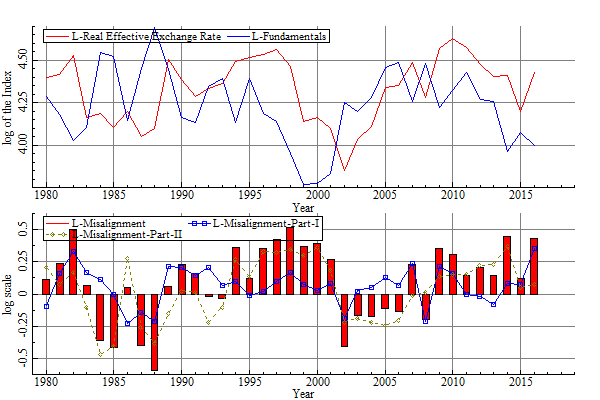
\includegraphics[width=8cm]{dadosEOP-brazil-graphic-misalignment-decomposition}

{\tiny{}L-Misalingment-Part-I is calculated from using ECM1.}{\tiny \par}

{\tiny{}L-Misalingment-Part-II is calculated from using ECM2}{\tiny \par}
\end{frame}

\begin{frame}{What we learned from the model with TB:}

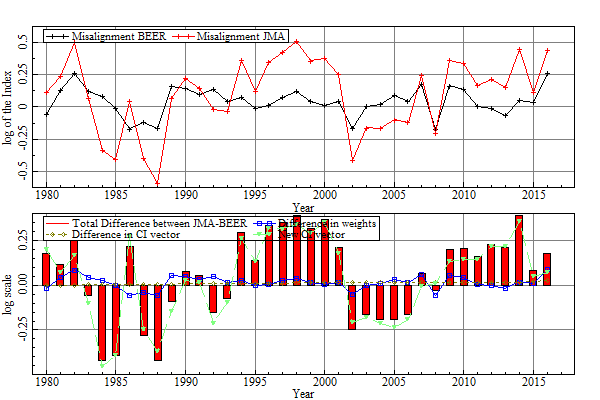
\includegraphics[width=8cm]{dadosEOP-brazil-graphic-difference-JMA_BEER-decomposition}
\end{frame}

\begin{frame}{Current account versus ECM-2:}

\includegraphics[width=10cm]{../../tb-NV/CA-PIB-BRAZIL}
\end{frame}


\subsection{Australian Case:}
\begin{frame}{TB and NFA:}

\textcolor{black}{\scriptsize{}}%
\begin{tabular}{rrrrrrrr}
\toprule 
\multicolumn{8}{l}{\textcolor{black}{\scriptsize{}Australia}}\tabularnewline
\midrule
\midrule 
\multicolumn{8}{c}{\textcolor{black}{\scriptsize{}System III: TB, NFA}}\tabularnewline
\midrule
\midrule 
\multicolumn{1}{c}{\textcolor{black}{\scriptsize{}Rank}} & \multicolumn{1}{c}{\textcolor{black}{\scriptsize{}Log-likelihood}} & \multicolumn{1}{c}{\textcolor{black}{\scriptsize{}Trace Test }} & \textcolor{black}{\scriptsize{}{[}p-value{]}} &  & \textcolor{black}{\scriptsize{}Max Test} & \textcolor{black}{\scriptsize{}{[}p-value{]}} & \tabularnewline
\midrule
\multicolumn{1}{c}{\textcolor{black}{\scriptsize{}0}} & \multicolumn{1}{c}{\textcolor{black}{\scriptsize{}-18.36}} & \multicolumn{1}{c}{\textbf{\textcolor{black}{\scriptsize{}19.95}}} & \multicolumn{1}{l}{\textbf{\textcolor{black}{\scriptsize{}{[}0.009{]}}}} & \multicolumn{1}{c}{\textbf{\textcolor{black}{\scriptsize{}{*}{*}{*}}}} & \multicolumn{1}{c}{\textbf{\textcolor{black}{\scriptsize{}19.06}}} & \multicolumn{1}{c}{\textbf{\textcolor{black}{\scriptsize{}{[}0.012{]}}}} & \multicolumn{1}{l}{\textbf{\textcolor{black}{\scriptsize{}{*}{*}}}}\tabularnewline
\multicolumn{1}{c}{\textcolor{black}{\scriptsize{}1}} & \multicolumn{1}{c}{\textcolor{black}{\scriptsize{}-9.03}} & \multicolumn{1}{c}{\textcolor{black}{\scriptsize{}1.29}} & \multicolumn{1}{l}{\textcolor{black}{\scriptsize{}{[}0.257{]}}} & \multicolumn{1}{c}{} & \multicolumn{1}{c}{\textcolor{black}{\scriptsize{}1.23}} & \multicolumn{1}{c}{\textcolor{black}{\scriptsize{}{[}0.268{]}}} & \multicolumn{1}{l}{}\tabularnewline
\multicolumn{1}{c}{\textcolor{black}{\scriptsize{}2}} & \multicolumn{1}{c}{\textcolor{black}{\scriptsize{}-8.38}} & \multicolumn{1}{c}{} & \multicolumn{1}{c}{} &  & \multicolumn{1}{c}{} & \multicolumn{1}{c}{} & \tabularnewline
\midrule
\multicolumn{8}{l}{\textcolor{black}{\scriptsize{}Model is a VAR(2) with a dummy for
2008 and 2009. }}\tabularnewline
\multicolumn{8}{l}{\textcolor{black}{\scriptsize{}Specification tests do not show evidence
against the null of non auto-correlation,}}\tabularnewline
\multicolumn{8}{l}{\textcolor{black}{\scriptsize{}homoskedasticity and normality.}}\tabularnewline
\end{tabular}{\scriptsize \par}
\end{frame}

\begin{frame}{LRER, NFA and fundamentals:}

\textcolor{black}{\scriptsize{}}%
\begin{tabular}{rrrrrrrr}
\toprule 
\multicolumn{8}{l}{\textcolor{black}{\scriptsize{}Australia}}\tabularnewline
\midrule
\midrule 
\multicolumn{8}{c}{\textcolor{black}{\scriptsize{}System II: LRER, NFA, LTOT, LBSGDP}}\tabularnewline
\midrule
\midrule 
\multicolumn{1}{c}{\textcolor{black}{\scriptsize{}Rank}} & \multicolumn{1}{c}{\textcolor{black}{\scriptsize{}Log-likelihood}} & \textcolor{black}{\scriptsize{}Trace Test} & \textcolor{black}{\scriptsize{}{[}p-value{]}} &  & \textcolor{black}{\scriptsize{}Max Test} & \textcolor{black}{\scriptsize{}{[}p-value{]}} & \tabularnewline
\midrule
\multicolumn{1}{c}{\textcolor{black}{\scriptsize{}0}} & \multicolumn{1}{c}{\textcolor{black}{\scriptsize{}264.56}} & \multicolumn{1}{c}{\textbf{\textcolor{black}{\scriptsize{}91.27}}} & \multicolumn{1}{c}{\textbf{\textcolor{black}{\scriptsize{}{[}0.000{]}}}} & \multicolumn{1}{l}{\textbf{\textcolor{black}{\scriptsize{}{*}{*}{*}}}} & \multicolumn{1}{c}{\textbf{\textcolor{black}{\scriptsize{}83.16}}} & \multicolumn{1}{c}{\textbf{\textcolor{black}{\scriptsize{}{[}0.000{]}}}} & \multicolumn{1}{l}{\textbf{\textcolor{black}{\scriptsize{}{*}{*}{*}}}}\tabularnewline
\multicolumn{1}{c}{\textcolor{black}{\scriptsize{}1}} & \multicolumn{1}{c}{\textcolor{black}{\scriptsize{}291.35}} & \multicolumn{1}{c}{\textbf{\textcolor{black}{\scriptsize{}37.68}}} & \multicolumn{1}{c}{\textbf{\textcolor{black}{\scriptsize{}{[}0.004{]}}}} & \textbf{\textcolor{black}{\scriptsize{}{*}{*}{*}}}\textcolor{black}{\scriptsize{} } & \multicolumn{1}{c}{\textbf{\textcolor{black}{\scriptsize{}34.33}}} & \multicolumn{1}{c}{\textbf{\textcolor{black}{\scriptsize{}{[}0.013{]}}}} & \textbf{\textcolor{black}{\scriptsize{}{*}{*}}}\textcolor{black}{\scriptsize{} }\tabularnewline
\multicolumn{1}{c}{\textcolor{black}{\scriptsize{}2}} & \multicolumn{1}{c}{\textcolor{black}{\scriptsize{}304.06}} & \multicolumn{1}{c}{\textcolor{black}{\scriptsize{}12.28}} & \multicolumn{1}{c}{\textcolor{black}{\scriptsize{}{[}0.145{]}}} &  & \multicolumn{1}{c}{\textcolor{black}{\scriptsize{}11.19}} & \multicolumn{1}{c}{\textcolor{black}{\scriptsize{}{[}0.203{]}}} & \tabularnewline
\multicolumn{1}{c}{\textcolor{black}{\scriptsize{}3}} & \multicolumn{1}{c}{\textcolor{black}{\scriptsize{}310.03}} & \multicolumn{1}{c}{\textcolor{black}{\scriptsize{}0.33}} & \multicolumn{1}{c}{\textcolor{black}{\scriptsize{}{[}0.565{]}}} & \textcolor{black}{\scriptsize{} } & \multicolumn{1}{c}{\textcolor{black}{\scriptsize{}0.3}} & \multicolumn{1}{c}{\textcolor{black}{\scriptsize{}{[}0.583{]}}} & \textcolor{black}{\scriptsize{} }\tabularnewline
\multicolumn{1}{c}{\textcolor{black}{\scriptsize{}4}} & \multicolumn{1}{c}{\textcolor{black}{\scriptsize{}310.20}} & \multicolumn{1}{c}{} & \multicolumn{1}{c}{} &  & \multicolumn{1}{c}{} & \multicolumn{1}{c}{} & \tabularnewline
\midrule
\multicolumn{8}{l}{\textcolor{black}{\scriptsize{}Model is a VAR(2) with a dummy for
2008 and 2009. }}\tabularnewline
\multicolumn{8}{l}{\textcolor{black}{\scriptsize{}Specification tests do not show evidence
against the null of non auto-correlation,}}\tabularnewline
\multicolumn{8}{l}{\textcolor{black}{\scriptsize{}homoskedasticity and normality.}}\tabularnewline
\end{tabular}{\scriptsize \par}
\end{frame}

\begin{frame}{LRER, NFA, TB and fundamentals:}

\textcolor{black}{\scriptsize{}}%
\begin{tabular}{llllllll}
\toprule 
\multicolumn{8}{c}{\textcolor{black}{\scriptsize{}Australia}}\tabularnewline
\midrule 
\multicolumn{8}{c}{\textcolor{black}{\scriptsize{}System I: LRER, NFA, TB, LTOT, LBSGDP}}\tabularnewline
\midrule
\midrule 
\multicolumn{1}{c}{\textcolor{black}{\scriptsize{}Rank}} & \multicolumn{1}{c}{\textcolor{black}{\scriptsize{}Log-likelihood}} & \textcolor{black}{\scriptsize{}Trace Test} & \textcolor{black}{\scriptsize{}{[}p-value{]}} &  & \textcolor{black}{\scriptsize{}Max Test} & \textcolor{black}{\scriptsize{}{[}p-value{]}} & \tabularnewline
\midrule
\multicolumn{1}{c}{\textcolor{black}{\scriptsize{}0}} & \multicolumn{1}{c}{\textcolor{black}{\scriptsize{}194.88}} & \multicolumn{1}{c}{\textbf{\textcolor{black}{\scriptsize{}124.82}}} & \multicolumn{1}{c}{\textbf{\textcolor{black}{\scriptsize{}{[}0.000{]}}}} & \multicolumn{1}{l}{\textbf{\textcolor{black}{\scriptsize{}{*}{*}{*}}}} & \multicolumn{1}{c}{\textbf{\textcolor{black}{\scriptsize{}64.87}}} & \multicolumn{1}{c}{\textbf{\textcolor{black}{\scriptsize{}{[}0.000{]}}}} & \multicolumn{1}{l}{\textbf{\textcolor{black}{\scriptsize{}{*}{*}{*}}}}\tabularnewline
\multicolumn{1}{c}{\textcolor{black}{\scriptsize{}1}} & \multicolumn{1}{c}{\textcolor{black}{\scriptsize{}227.32}} & \multicolumn{1}{c}{\textbf{\textcolor{black}{\scriptsize{}59.95}}} & \multicolumn{1}{c}{\textbf{\textcolor{black}{\scriptsize{}{[}0.002{]}}}} & \multicolumn{1}{l}{\textbf{\textcolor{black}{\scriptsize{}{*}{*}{*}}}} & \multicolumn{1}{c}{\textbf{\textcolor{black}{\scriptsize{}25.9}}} & \multicolumn{1}{c}{\textbf{\textcolor{black}{\scriptsize{}{[}0.079{]}}}} & \multicolumn{1}{l}{\textbf{\textcolor{black}{\scriptsize{}{*}}}}\tabularnewline
\multicolumn{1}{c}{\textcolor{black}{\scriptsize{}2}} & \multicolumn{1}{c}{\textcolor{black}{\scriptsize{}240.27}} & \multicolumn{1}{c}{\textbf{\textcolor{black}{\scriptsize{}34.05}}} & \multicolumn{1}{c}{\textbf{\textcolor{black}{\scriptsize{}{[}0.014{]}}}} & \textbf{\textcolor{black}{\scriptsize{}{*}{*}}}\textcolor{black}{\scriptsize{} } & \multicolumn{1}{c}{\textbf{\textcolor{black}{\scriptsize{}21.54}}} & \multicolumn{1}{c}{\textbf{\textcolor{black}{\scriptsize{}{[}0.042{]}}}} & \textbf{\textcolor{black}{\scriptsize{}{*}{*}}}\textcolor{black}{\scriptsize{} }\tabularnewline
\multicolumn{1}{c}{\textcolor{black}{\scriptsize{}3}} & \multicolumn{1}{c}{\textcolor{black}{\scriptsize{}251.04}} & \multicolumn{1}{c}{\textcolor{black}{\scriptsize{}12.5}} & \multicolumn{1}{c}{\textcolor{black}{\scriptsize{}{[}0.135{]}}} & \textcolor{black}{\scriptsize{} } & \multicolumn{1}{c}{\textcolor{black}{\scriptsize{}12.28}} & \multicolumn{1}{c}{\textcolor{black}{\scriptsize{}{[}0.100{]}}} & \textcolor{black}{\scriptsize{} }\tabularnewline
\multicolumn{1}{c}{\textcolor{black}{\scriptsize{}4}} & \multicolumn{1}{c}{\textcolor{black}{\scriptsize{}257.18}} & \multicolumn{1}{c}{\textcolor{black}{\scriptsize{}0.22}} & \multicolumn{1}{c}{\textcolor{black}{\scriptsize{}{[}0.639{]}}} &  & \multicolumn{1}{c}{\textcolor{black}{\scriptsize{}0.22}} & \multicolumn{1}{c}{\textcolor{black}{\scriptsize{}{[}0.639{]}}} & \tabularnewline
\multicolumn{1}{c}{\textcolor{black}{\scriptsize{}5}} & \multicolumn{1}{c}{\textcolor{black}{\scriptsize{}257.29}} & \multicolumn{1}{c}{} & \multicolumn{1}{c}{} &  & \multicolumn{1}{c}{} & \multicolumn{1}{c}{} & \tabularnewline
\midrule
\multicolumn{8}{l}{\textcolor{black}{\scriptsize{}Model is a VAR(2) with a dummy for
2008 and 2009. }}\tabularnewline
\multicolumn{8}{l}{\textcolor{black}{\scriptsize{}Specification tests do not show evidence
against the null of non auto-correlation,}}\tabularnewline
\multicolumn{8}{l}{\textcolor{black}{\scriptsize{}homoskedasticity and normality.}}\tabularnewline
\end{tabular}{\scriptsize \par}
\end{frame}

\begin{frame}{Restricted Model: LRER, NFA and TB:}
\begin{itemize}
\item Rela��es de cointegra��o estimadas:
\end{itemize}
\textrm{
\begin{eqnarray*}
ECM1_{t} & = & RER_{t}-0.41421*NFA_{t}-0.31740TOT_{t}
\end{eqnarray*}
}

\textrm{
\begin{eqnarray*}
ECM2_{t} & = & RER_{t}-0.40935*LBSGDP{}_{t}
\end{eqnarray*}
}

\textrm{
\begin{eqnarray*}
ECM3_{t} & = & TB_{t}-2.0980*NFA_{t}
\end{eqnarray*}
}
\end{frame}

\begin{frame}{Exchange Rate Misalignment Estimate:}


\includegraphics[width=10cm]{../../tb-NV/AUSTRALIA-CODES/dadosEOP-australia-graphic-misalignment-decomposition}
\end{frame}

\begin{frame}{What we learned from the model with TB:}


\includegraphics[width=10cm]{../../tb-NV/dadosEOP-australia-graphic-difference-JMA_BEER-decomposition}
\end{frame}


\section{What else we are working on...}
\begin{frame}{Global VAR:}
\begin{itemize}
\item Exchange rate equilibrium may depend on a external common factor;
\item What is going on in our main trading patterns may be important as
well;
\item Treat economies as detached entities may not be the best approach;
\end{itemize}
\end{frame}
%
\begin{frame}{But}
\begin{itemize}
\item Analysts has to face curse of dimensionality;
\item GVAR seems to be a good option;
\item Working Paper on that available at SSRN (\href{https://papers.ssrn.com/sol3/papers.cfm?abstract_id=2364508}{link});
\item No good evidence of long run links
\begin{itemize}
\item Mar�al \cite{marccal2014exchange} (\href{http://bibliotecadigital.fgv.br/ojs/index.php/rbe/article/view/9677}{link});
\end{itemize}
\end{itemize}
\end{frame}

\begin{frame}{FAVECM:}
\begin{itemize}
\item Another possibility is to work with high dimension models;
\begin{itemize}
\item Banerjee \cite{banerjee2014structural}
\end{itemize}
\item It possible to deal with a higher information set;
\end{itemize}
\end{frame}

\begin{frame}{Mixed Frequency Data:}
\begin{itemize}
\item Real effective exchange rate is available in multiple frequencies;
\item It would interest to use all information available to estimate and
access misalignment;
\end{itemize}
\end{frame}


\appendix

\section*{}

\bibliographystyle{plain}
\bibliography{refs}

\end{document}
